\usetikzlibrary{arrows.meta,calc}
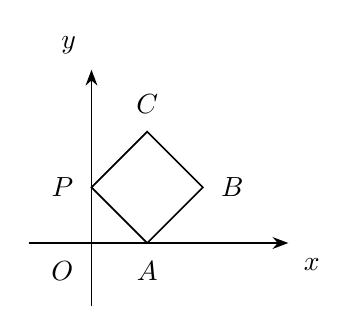
\begin{tikzpicture}[x=1cm,y=1cm,line width=.6pt,font=\normalsize,>=Stealth]
\coordinate (O) at (0,0);
\coordinate (P) at (0,0.70710678);
\coordinate (A) at (0.70710678,0);
\coordinate (B) at (1.41421356,0.70710678);
\coordinate (C) at (0.70710678,1.41421356);
\coordinate (XaxisL) at (-0.8,0);
\coordinate (XaxisR) at (2.5,0);
\coordinate (YaxisB) at (0,-0.8);
\coordinate (YaxisT) at (0,2.2);
\draw[->] (XaxisL) -- (XaxisR);
\draw[->] (YaxisB) -- (YaxisT);
\draw (P) -- (A) -- (B) -- (C) -- cycle;
\node[below left=3pt] at (O) {$O$};
\node[left=3pt] at (P) {$P$};
\node[below=3pt] at (A) {$A$};
\node[right=3pt] at (B) {$B$};
\node[above=3pt] at (C) {$C$};
\node[below right=2pt] at (XaxisR) {$x$};
\node[above left=2pt] at (YaxisT) {$y$};
\end{tikzpicture}
